\subsection{Mechanizmy Kubernetes stojące za Lupus}
Niniejsza praca zakłada znajomość czytelnika platformy Kubernetes na podstawowym poziomie.

\subsubsection{Kontroler}
Działanie Kubernetes opiera się na zamkniętej pętli sterowania \footnote{https://kubernetes.io/docs/concepts/architecture/controller/}. \textbf{Aktualny Stan} systemu zapisany jest w bazie etcd. \textbf{Stan Pożądany} wyrażony jest poprzez pliki manifestacyjne. Każdy \textit{Obiekt API} posiada swoją sekcję \texttt{spec}, która określa jego pożądany stan. Każdy obiekt ma swój kontroler, który rekoncyliuję aktualny stan do stan pożądanego. Kontroler jest to proces działający w warstwie sterowania Kubernetes. Każdy typ (ang. \textit{Kind}) wbudowanych zasobów (ang. \textit{buil-in resources}) posiada kontroler opracowany przez zespół Kubernetes. Kontrolery każdego typu zasobu działają w podzie \texttt{kube-controller-manager}. 

\begin{figure}[!h]
    \centering 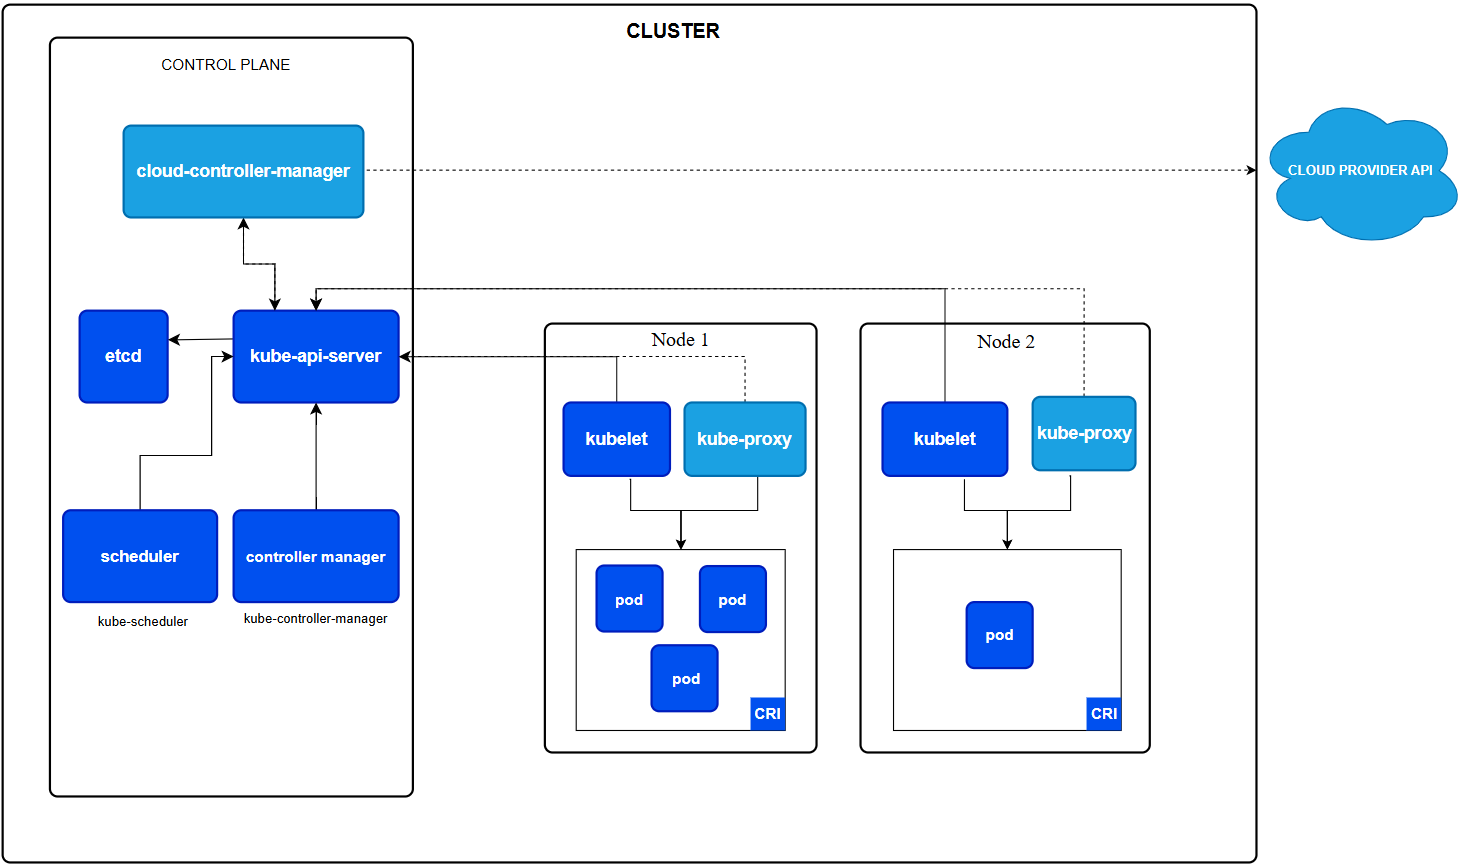
\includegraphics[width=1\linewidth]{42-k8s-arch.png}
    \caption{Architektura Kubernetes. Źródło: \url{https://kubernetes.io/docs/concepts/architecture/}}\label{fig:42-k8s-arch}
\end{figure}

Przepływ pracy kontrolera pokazano na rysunku \ref{fig:42-flow}. Gdy \texttt{kube-api-server} otrzymuje żądanie zmiany danego obiektu API, zanim zleci jego utrwalenie w bazie etcd, wykonuje tzw. webhooki do kontrolera danego obiektu. Webhooki nie są jednakże istotne z punktu widzenia niniejszej pracy dyplomowej. Po dokonaniu zmian w obiekcie kontroler zostaje o nich poinformowany. Jego głównym zadaniem jest rekoncyliacja, czyli porównanie aktualnego stanu obiektu ze stanem pożądanym. Kontroler zawiera logikę rekoncyliacyjną, która dąży do doprowadzenia stanu aktualnego do stanu pożądanego. Realizacja logiki rekoncyliacji często wiąże się z wykonywaniem różnych akcji w innych częściach klastra, takich jak skalowanie zasobów, tworzenie nowych instancji lub modyfikacja konfiguracji.

\begin{figure}[!h]
    \centering 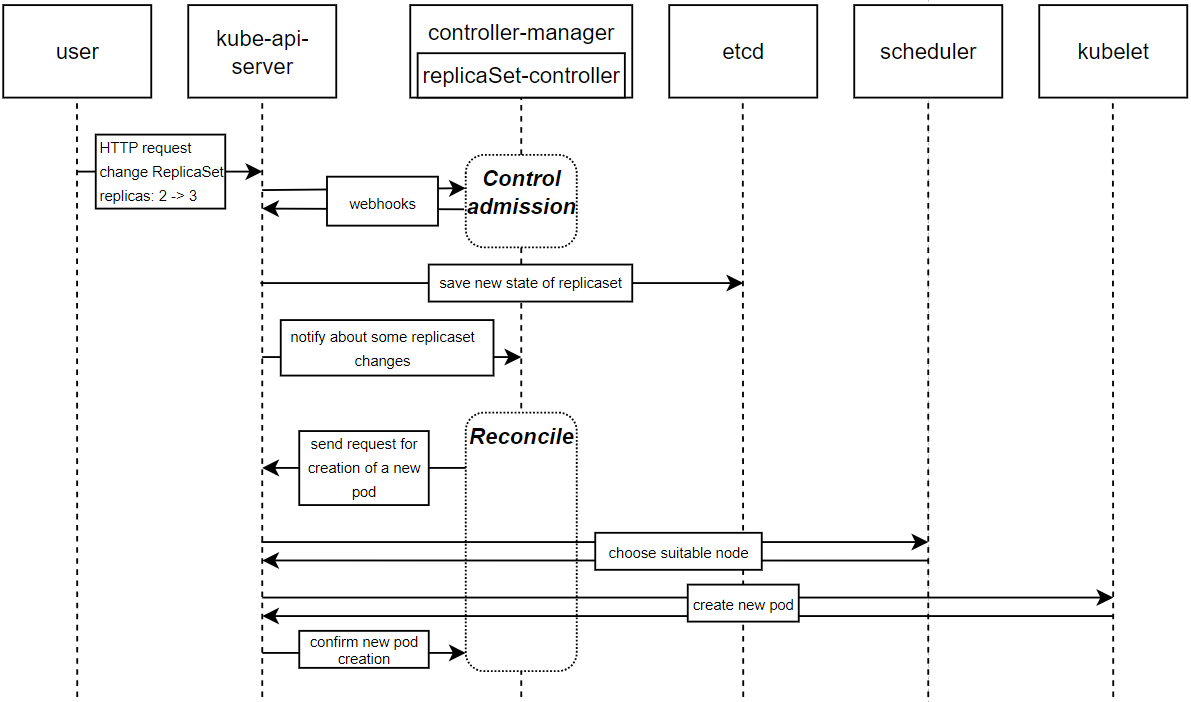
\includegraphics[width=1\linewidth]{42-flow.png}
    \caption{Flow pracy kontrolera. Źródło: Opracowanie własne.}\label{fig:42-flow}
\end{figure}

\subsubsection{Zasoby własne} 

\hyperlink{def:zasoby-wlasne}{\textit{Zasoby własne} (ang. \textit{Custom Resources})} rozszerzają zasoby wbudowane (ang. \textit{buit-in resources}) o niestandardowe typy, zdefiniowane przez użytkownika. Najczęściej tworzone są w celu zarządzania konfiguracją skomplikowanych lub stanowych aplikacji, tam gdzie wbudowane typy zasobów, takie jak Pody, Wdrożenia (Deployments) czy Serwisy (Services), nie są wystarczające. Aby utworzyć nowy typ zasobu, należy:
\begin{enumerate}
    \item Zdefiniować plik manifestacyjny YAML typu Custom Resource Definition (CRD).
    \item Zaaplikować CRD w klastrze Kubernetes.
\end{enumerate}

Po pomyślnym dodaniu definicji możliwe jest tworzenie obiektów nowego typu, które będą zarządzane przez Kubernetes w taki sam sposób jak zasoby wbudowane.

\subsubsection{Operatory}

Operator to kolejny mechanizm rozszerzania Kubernetes. Kiedy tworzymy Zasoby Własne (ang. \textit{Custom Resources}), możemy również implementować dla nich kontrolery. Takie podejście nazywane jest "wzorem operatora" ("operator-pattern"). Nazwa ta wynika z faktu, że operator pełni funkcję automatycznego zarządcy, zastępując człowieka, który w przeciwnym razie musiałby ręcznie zarządzać wdrożeniem i konfiguracją aplikacji wymagającej Zasobów Własnych. Lupus wykorzystuje zasoby własne w celu reprezentacji zewnętrznego bytu, nie skomplikowanej aplikacji.
\subsubsection{Kubebuilder}

Kubebuilder jest frameworkiem programistycznym do tworzenia \textit{Zasobów Własnych} oraz ich \textit{Operatorów}. Pozwala zaprogramować sekcje przepływu pracy kontrolera zaznaczone na rysunku \ref{fig:42-flow2} jasno czerwonym kolorem.


\begin{figure}[!h]
    \centering 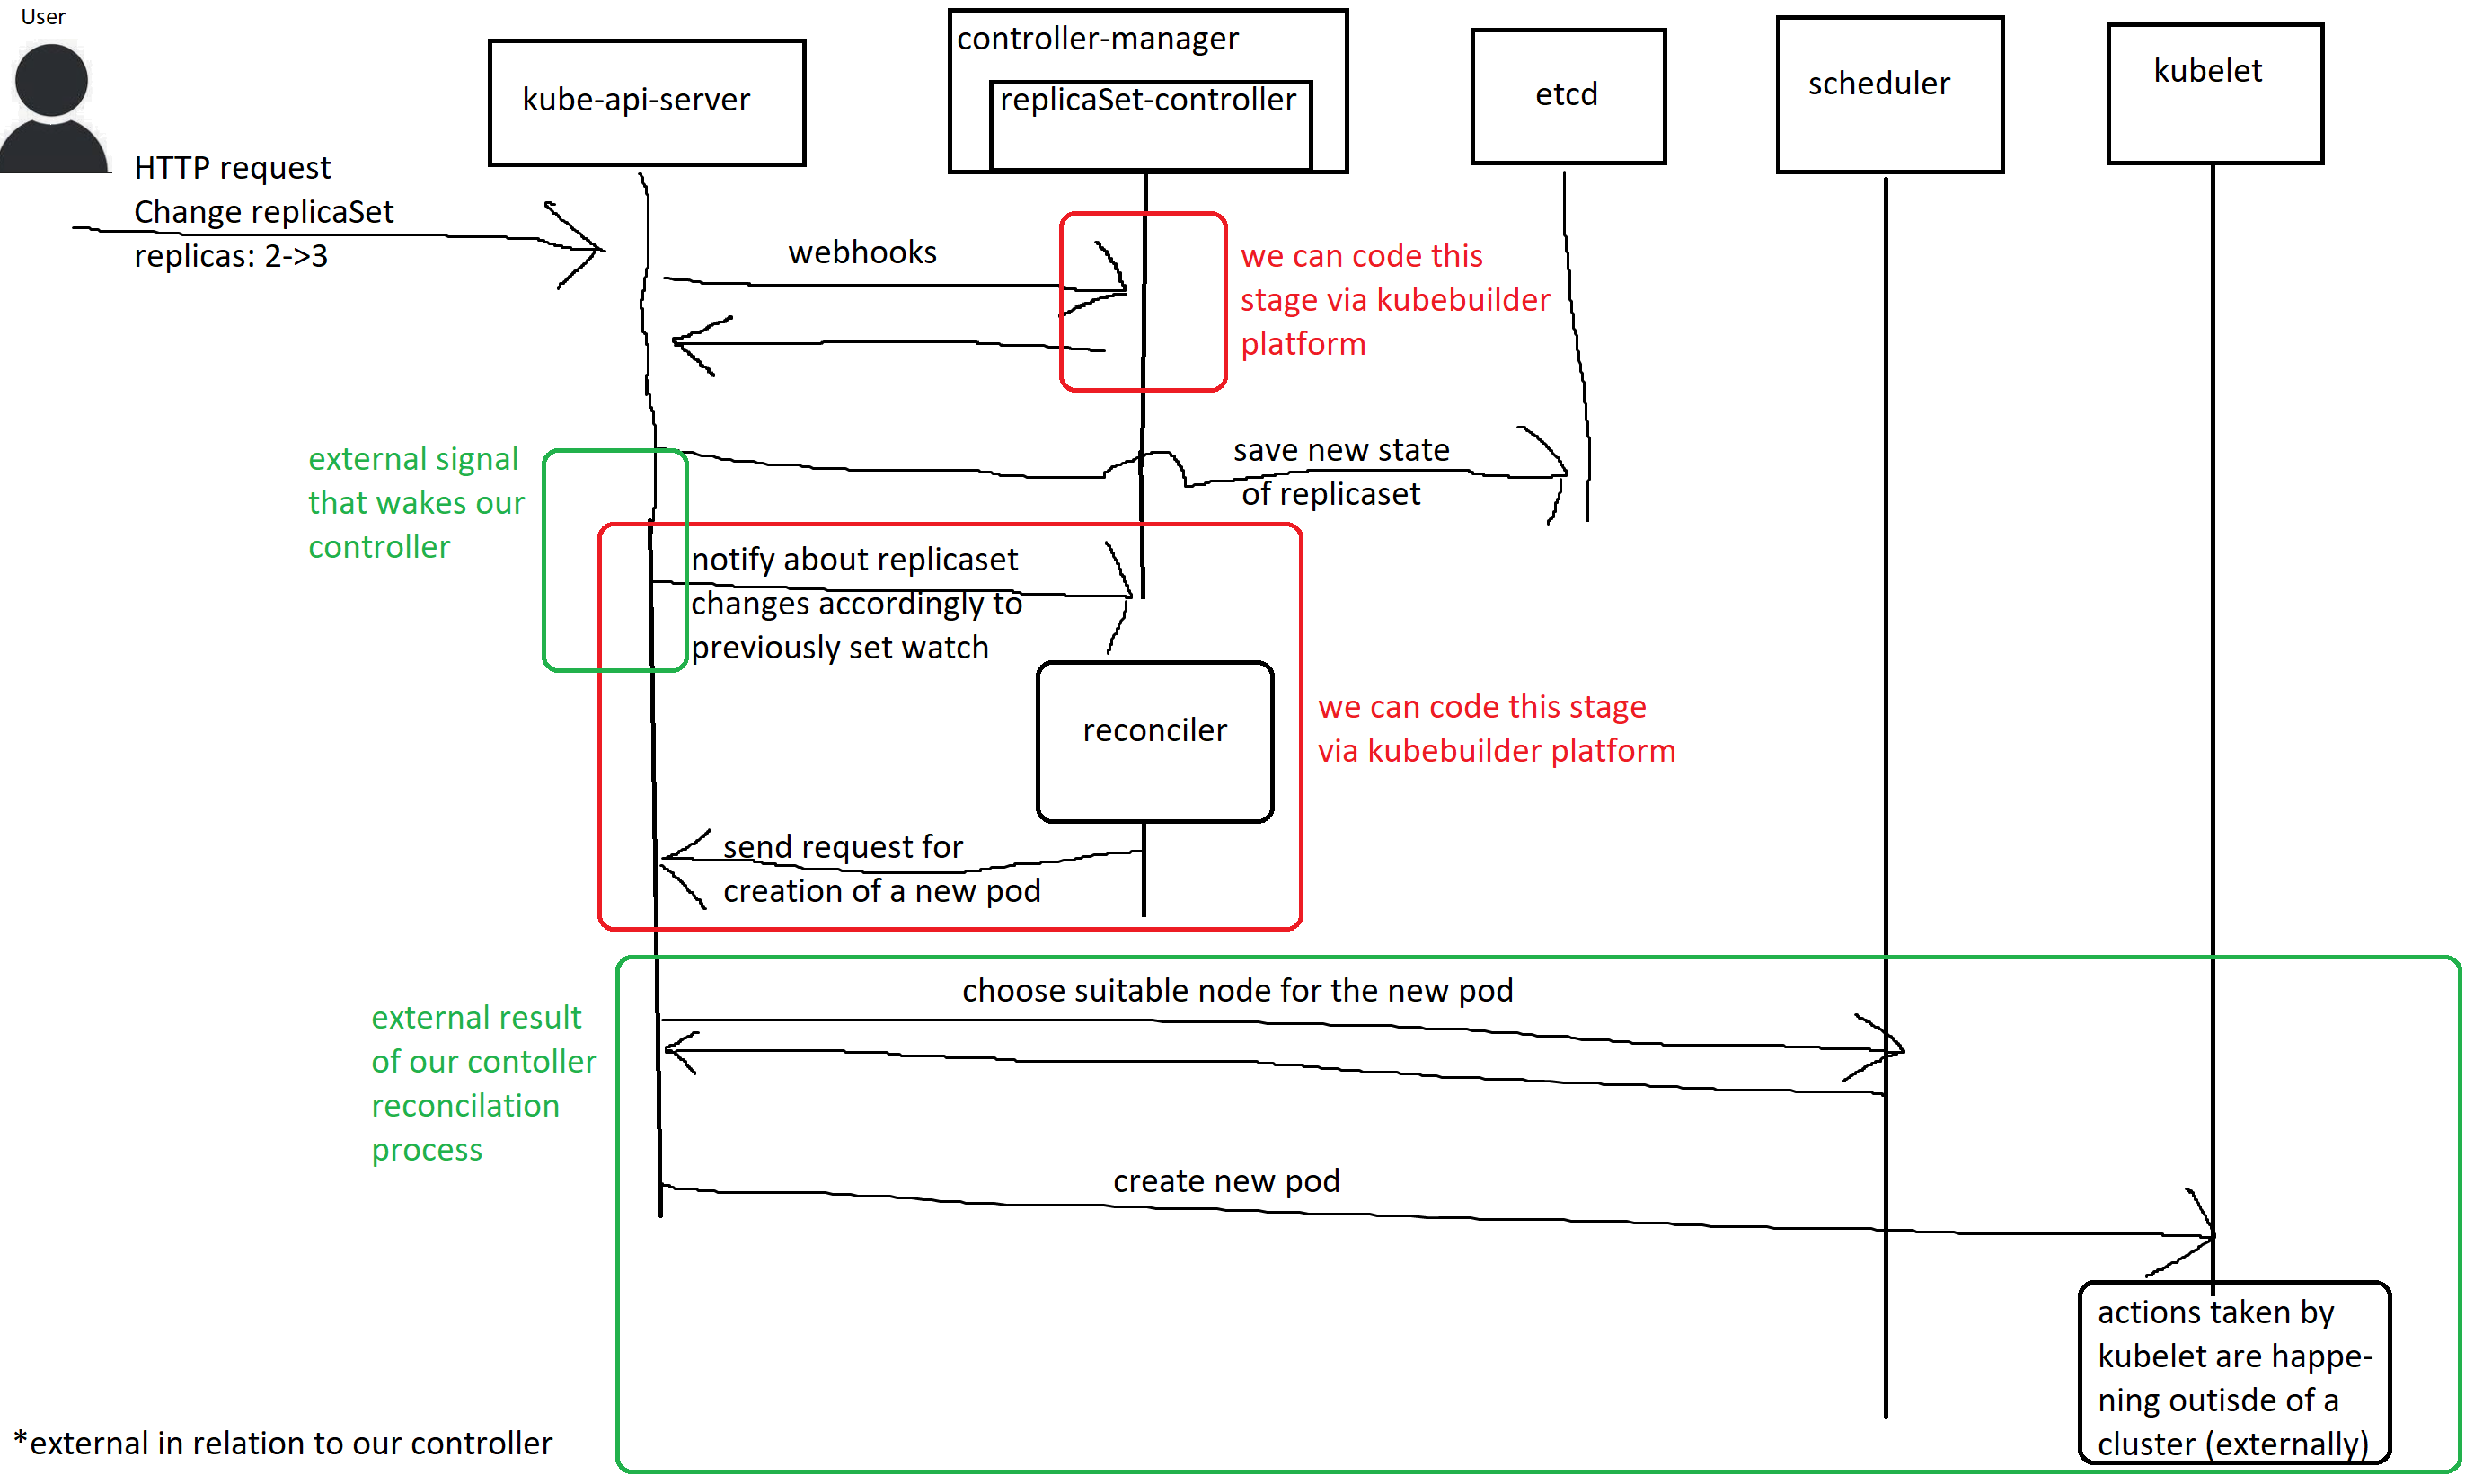
\includegraphics[width=1\linewidth]{42-flow2.png}
    \caption{Zaznaczenie możliwych do zaprogramowania elementów flow pracy kontrolera. Źródło: Opracowanie własne.}\label{fig:42-flow2}
\end{figure}